\begin{figure}[t]
  \centering
  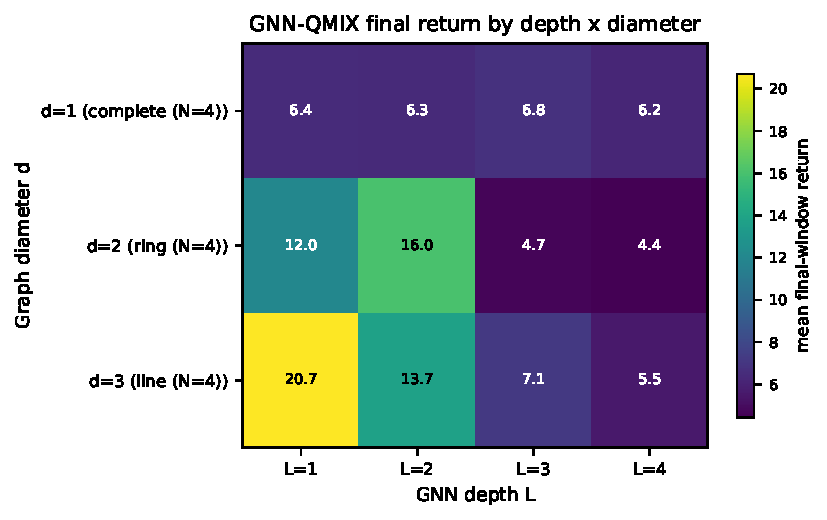
\includegraphics[width=0.5\linewidth]{figures/phase4__heatmap_final_return.pdf}
  \caption{Phase 4: GNN-QMIX final-window mean return as a function of GNN depth $L$ and coordination graph diameter $d$. Cells along the diagonal correspond to depth--diameter alignment ($L \approx d$), the H3 prediction.}
  \Description{Heat map with GNN depth L on the x-axis (1 to 4) and graph
  diameter d on the y-axis (1, 2, 3); cell color encodes final-window mean
  return from low (dark) to high (bright). The two leftmost columns (L=1,2)
  are bright across all diameters; the two rightmost columns (L=3,4) are
  uniformly dark, showing a sharp over-depth cliff independent of diameter.}
  \label{fig:phase4_heatmap}
\end{figure}

\begin{table}[t]
  \centering
  \small
  \caption{H3 (depth--diameter alignment) per-diameter test, pre-registered criteria: (a) the depth curve must be non-flat (relative range $\geq 10\%$ of peak), AND (b) the argmax depth $L^*$ must satisfy $|L^* - d| \leq 1$. Per-diameter passes: 1/3.}
  \label{tab:phase4_h3}
  \begin{tabular}{rrrrc}
    \toprule
    $d$ & $L^*$ (argmax) & Peak return & rel.\ range & pass \\
    \midrule
    1 & 3 & 6.77 & 0.09 & $\times$ \\
2 & 2 & 16.03 & 0.72 & \checkmark \\
3 & 1 & 20.71 & 0.73 & $\times$ \\
    \bottomrule
  \end{tabular}
\end{table}
